\documentclass[tikz,border=2pt]{standalone}

\usepackage{pgfplots}
\pgfplotsset{compat=1.18}

\begin{document}
	
	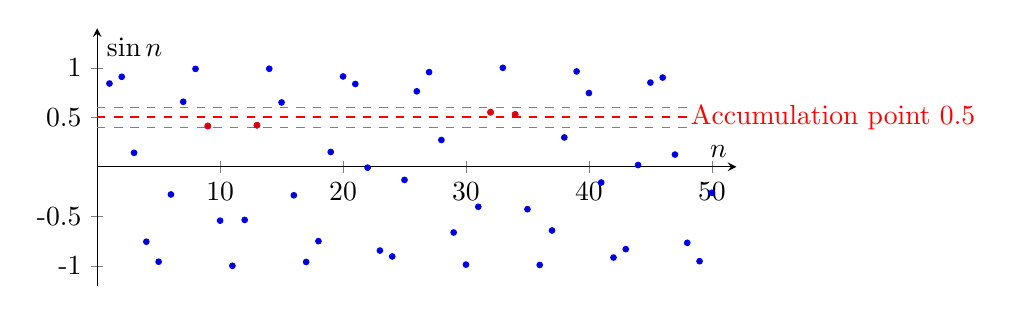
\begin{tikzpicture}
		\begin{axis}[
			xlabel=\( n \),
			ylabel=\( \sin n \),
			ytick={-1, -0.5, 0, 0.5, 1},
			yticklabels={-1, -0.5, 0, 0.5, 1},
			axis lines=center,
			ymin=-1.2,
			ymax=1.4,
			xmin=0,
			xmax=52,
			width=0.8\textwidth,
			height=0.4\textwidth,
			clip=false,
			]
			
			\addplot+[only marks, blue, mark=*, mark size=1pt, samples at={1,...,50}] {sin(deg(x))};
			
			% Specific points marked in red
			\addplot+[only marks, red, mark=*, mark size=1pt, samples at={9,13,32,34}] {sin(deg(x))};
			
			% Dashed lines representing the interval [0.4, 0.6]
			\addplot[color= red, thick, dashed, domain=0:48] {0.5};
			\addplot[color= gray, dashed, domain=0:48] {0.4};
			\addplot[color= gray, dashed, domain=0:48] {0.6};
			
			\node[right, color= red] at (axis cs: 47.5, 0.5) {Accumulation point $0.5$};
		\end{axis}
	\end{tikzpicture}
	
\end{document}